\documentclass[../report.tex]{subfiles}
\begin{document}
\paragraph*{}Trong mật mã học, MD5 (viết tắt của tiếng Anh Message-Digest algorithm 5, giải thuật Tiêu hóa tin 5) là một hàm 
băm mật mã học được sử dụng phổ biến với giá trị Hash dài 128-bit. Là một chuẩn Internet (RFC 1321), MD5 đã được dùng trong 
nhiều ứng dụng bảo mật, và cũng được dùng phổ biến để kiểm tra tính toàn vẹn của tập tin. 
Một bảng băm MD5 thường được diễn tả bằng một số hệ thập lục phân 32 ký tự.
MD5 được thiết kế bởi Ronald Rivest vào năm 1991 để thay thế cho hàm băm trước đó, MD4. 
Vào năm 1996, người ta phát hiện ra một lỗ hổng trong MD5; 
trong khi vẫn chưa biết nó có phải là lỗi nghiêm trọng hay không, những chuyên gia mã hóa bắt đầu đề nghị 
sử dụng những giải thuật khác, như SHA-1 (khi đó cũng bị xem là không an toàn). Trong năm 2004, nhiều lỗ hổng hơn bị 
khám phá khiến cho việc sử dụng giải thuật này cho mục đích bảo mật đang bị đặt nghi vấn. 
\paragraph*{} Yêu cầu của thuật toán mã hõa này được mô tả đơn giản như sau:
\begin{itemize}
    \item \textbf{Input: } thông điệp với độ dài bất kỳ (Ở đây đặt độ dài thông điệp tối đa là 20 bit)
    \item \textbf{Output: } giá trị băm (message digest) 128 bits
\end{itemize}

\subsection{Giải thuật}
\paragraph*{}Giải thuật gồm 5 bước thao tác trên khối 512 bits.
\subsubsection{Tạo block}
MD5 chuyển một đoạn thông tin chiều dài thay đổi thành 
một kết quả chiều dài không đổi 128 bit. Mẩu tin đầu vào được chia thành từng đoạn 512 bit; mẩu tin sau đó được độn sao 
cho chiều dài của nó chia chẵn cho 512. Công việc độn vào như sau: đầu tiên một bit đơn, 1, được gắn vào cuối mẩu tin. 
Tiếp theo là một dãy các số zero sao cho chiều dài của mẩu tin lên tới 64 bit ít hơn so với bội số của 512. 
Những bit còn lại được lấp đầy bằng một số nguyên 64-bit đại diện cho chiều dài của mẩu tin gốc với chú ý:
\begin{itemize}
    \item Độ dài của khối dữ liệu ban đầu được biểu diễn dưới dạng nhị phân 64-bit và được thêm vào 64 bit cuối của block theo thứ tự từ byte thấp tới byte cao.
    \item Nếu độ dài của khối dữ liệu ban đầu > $2^{64}$, chỉ 64 bits thấp được sử dụng, nghĩa là giá trị được thêm vào bằng K mod $2^{64}$.
\end{itemize}

\begin{figure}[H]
    \centering
    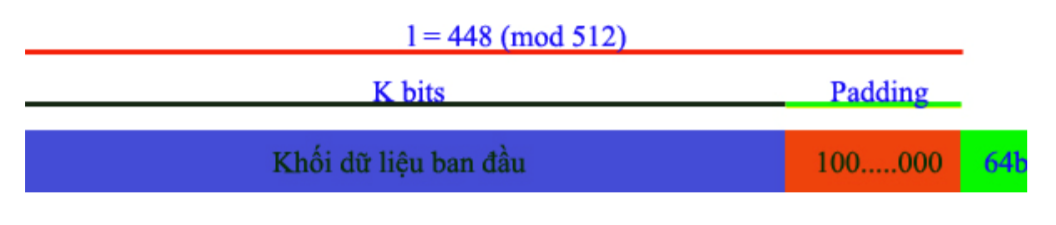
\includegraphics[width=\textwidth]{figures/block.png}
    \caption{Tạo block 512 bit cho dữ liệu nhập vào}
\end{figure}
Kết quả ta thu được khối dữ liệu có độ dài là bội của 512. Khối dữ liệu được biểu diễn:
\begin{itemize}
    \item Bằng một dãy L khối 512-bit $Y_0, Y_1,…, Y_{L-1}$
    \item Bằng một dãy N từ (word) 32-bit $M_0, M_1, M_{N-1}$. Vậy N = L x 16
\end{itemize}
\begin{figure}[H]
    \centering
    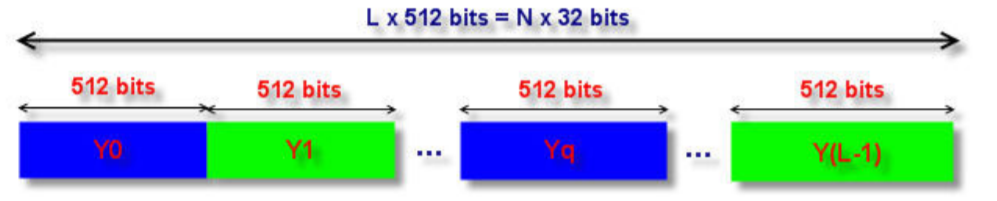
\includegraphics[width=\textwidth]{figures/blockCom.png}
    \caption{Khối 512 sau khi tạo xong}
\end{figure}
\subsubsection{Khởi tạo bộ đệm MD}
Một bộ đệm 128-bit được dùng lưu trữ các giá trị băm trung
gian và kết quả. Bộ đệm được biểu diễn bằng 4 thanh ghi 32-
bit (A, B, C, D) với các giá trị khởi tạo ở dạng little-endian (byte có trọng
số nhỏ nhất trong từ nằm ở địa chỉ thấp nhất) như sau:
    \begin{itemize}
        \item $A_0$ = 0x67452301 
        \item $B_0$ = 0xefcdab89 
        \item $C_0$ = 0x98badcfe   
        \item $D_0$ = 0x10325476   
    \end{itemize}

\subsubsection{Xử lý các khối dữ liệu 512 bit}
Trọng tâm của giải thuật đó là hàm xử lý các khối tin 512-bit (hàm nén), mỗi khối xác định một trạng thái. Quá trình xử lý khối tin 
bao gồm bốn giai đoạn giống nhau, gọi là vòng; mỗi vòng gồm có 16 tác vụ giống nhau dựa trên hàm phi tuyến F, cộng mô đun, và dịch trái. 
Hình vẽ mô tả một tác vụ trong một vòng. Có 4 khả năng cho hàm F; mỗi cái được dùng khác nhau cho mỗi vòng:

\begin{figure}[H]
    \centering
    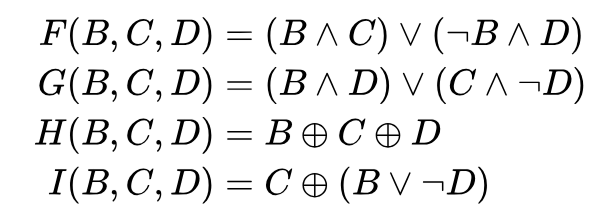
\includegraphics[width=9cm]{figures/F.png}
    \caption{Các hàm luận lý trong mỗi vòng}
\end{figure}

\begin{figure}[H]
    \centering
    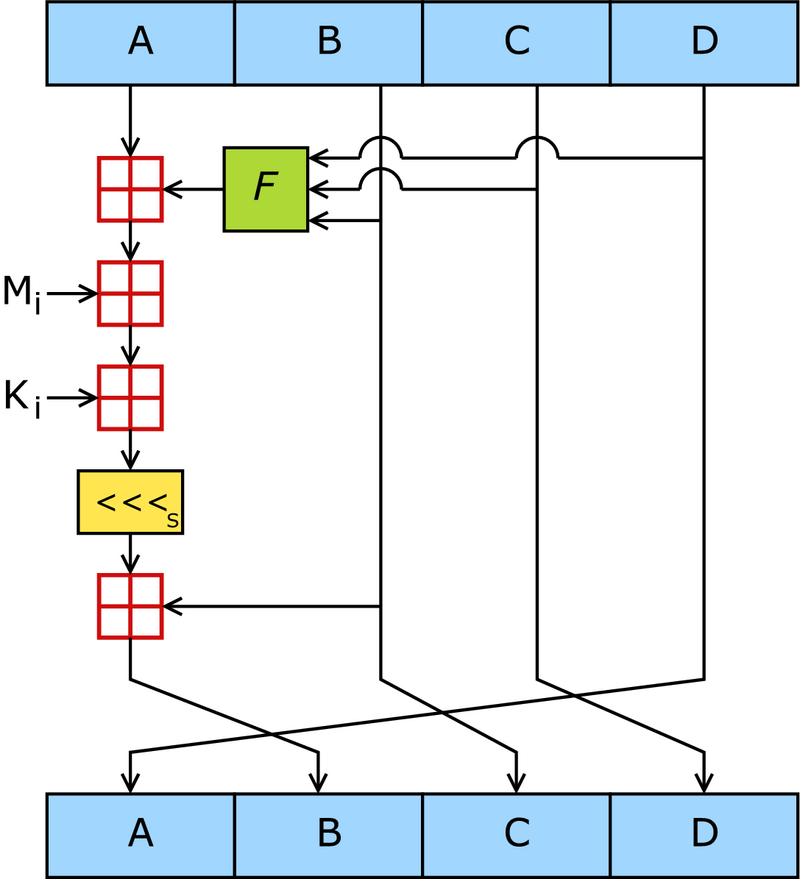
\includegraphics[width=9cm]{figures/round.png}
    \caption{Các thao tác được thực hiện trong một vòng }
\end{figure}

\subsection{Mã giả}
Thuật toán MD5 được thực hiện theo thuật toán sau, tất cả các giá trị đều ở dạng little-edian:
\begin{figure}[H]
    \centering
    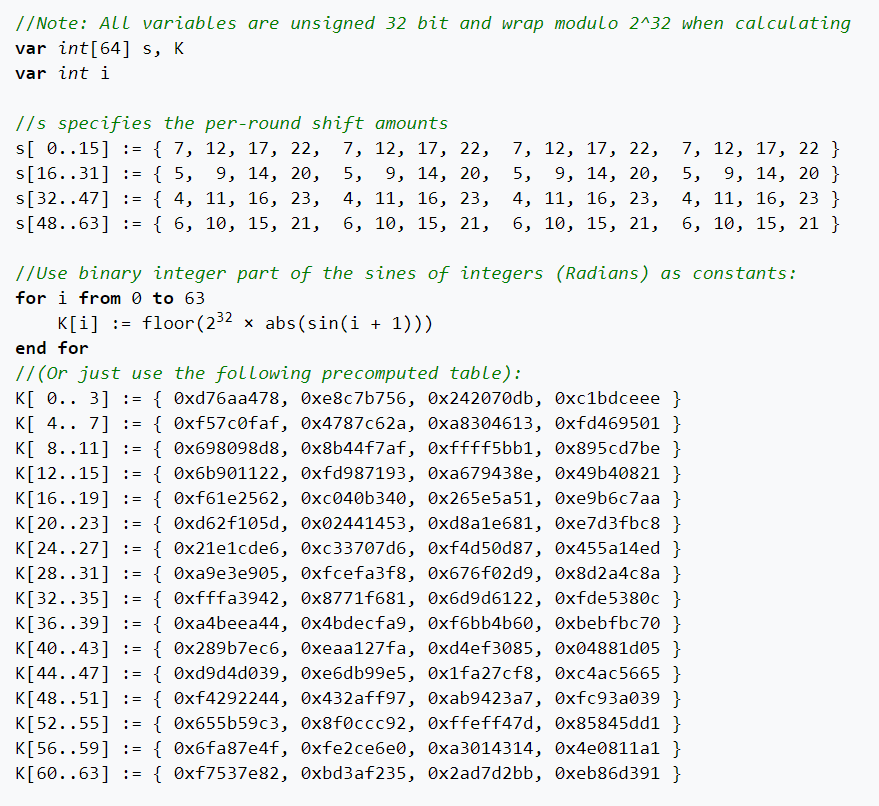
\includegraphics[width=\textwidth]{figures/al.png}
\end{figure}
\begin{figure}[H]
    \centering
    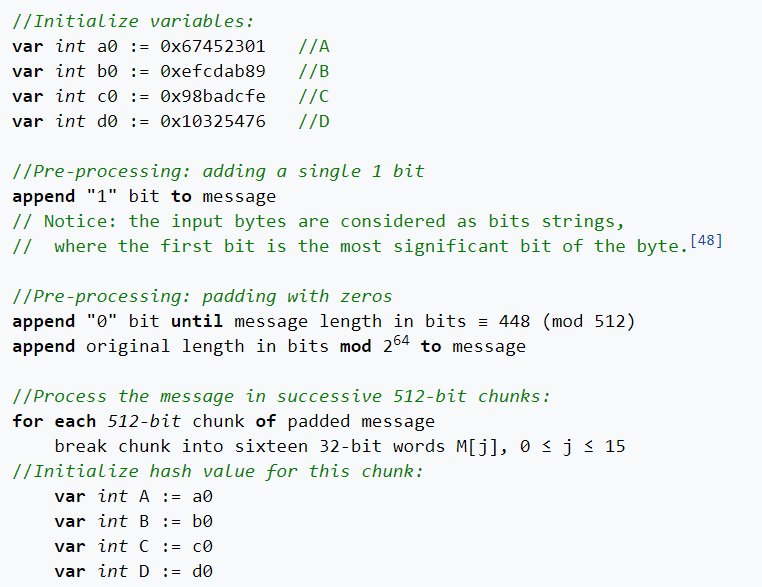
\includegraphics[width=\textwidth]{figures/al2.png}
\end{figure}
\begin{figure}[H]
    \centering
    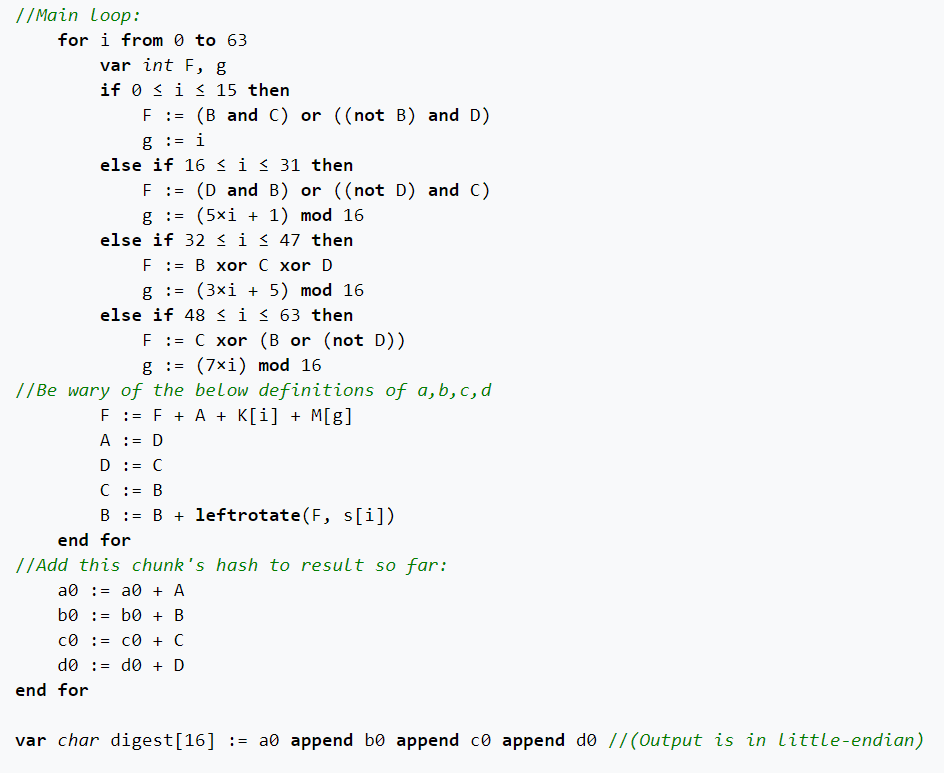
\includegraphics[width=\textwidth]{figures/al3.png}
\end{figure}

Một chút cải tiến cho thuật toán đó là thay thế hàm F ở hai vòng đầu:
\begin{itemize} 
    \item (0  <= i <= 15): F:= D \textbf{xor} (B \textbf{and} (C \textbf{xor} D))
    \item (16 <= i <= 31): F:= C \textbf{xor} (D \textbf{and} (B \textbf{xor} C))
\end{itemize}

\end{document}
